\section{Systematic uncertainties}
%%%%%%%%%%%%%%%%%%%%%%%%%%%%%%%%%%%%%%%%%%%%%%%%%%%%%%%%%%%%%%%%%%%%%%
\label{sec:Systematics}

Systematic uncertainties play an important role in this analysis where
no strong mass peak is expected due to the presence of undetected
neutrinos in the final state. They arise from three sources: background predictions, experimental measurements, and theoretical uncertainties. One of the most important sources is the normalization of the backgrounds that are estimated on data control samples whenever is possible.

The systematic uncertainties can affect the measured signal strengths in different ways. The uncertainties on the background predictions can be divided in those affecting the background cross section, the (\mll, \mt) shape or both. As an example, systematic uncertainties changing the background cross section are the ones related to the background data-driven estimation, while the b tagging uncertainties only have an effect on the (\mll, \mt) shape. Uncertainties such as lepton energy scale can instead affect both normalization and shape. Also, uncertainties affecting the signal (\mll, \mt) shape reflect on an uncertainty on the measured signal strength. 

A summary of the main sources of systematic uncertainty and the corresponding estimate is reported in Table~\ref{tab:Systematics}. A brief description of each source of systematic uncertainty is discussed in the following sections.

The uncertainties related to the unfolding procedure are treated separately and are discussed in Sec.~\ref{sec:uncunf}.

\begin{table}[!htb]
\small{
  \begin{center}
  \caption{Main sources of systematic uncertainties and their estimate. The
  first category reports the uncertainties on the normalization of background
  contributions. The experimental and theoretical uncertainties refer to the
  effect on signal yields. A range is specified if the uncertainty varies
  across the $\pth$ bins.}
  \label{tab:Systematics}
  \begin{tabular}{cc}
  \toprule
  \multicolumn{2}{c} {\bf{Uncertainties in backgrounds contributions}} \\
  \midrule
  Source  & Uncertainty \\
  \midrule
  $\rm{t\bar{t}}$, tW      & 20--50$\%$ \\
  W+jets              & $40\%$ \\
  WZ, ZZ              & $4\%$ \\
  W$\gamma^{*}$, W$\gamma$  & $30\%$ \\
  \toprule
  \multicolumn{2}{c} {\bf{Effect of the experimental uncertainties on the signal and background yields}}\\
  \midrule
  Source & Uncertainty\\
  \midrule
  Integrated luminosity        & $2.6\%$ \\
  Trigger efficiency           & 1--2$\%$\\
  Lepton reconstruction and identification & 3--4$\%$\\
  Lepton energy scale          & 2--4$\%$ \\
  \MET modelling          & $2\%$ \\
  Jet energy scale             & $10\%$ \\
  Pileup multiplicity          & $2\%$ \\
  b mistag modelling	       & $3\%$ \\	
  \toprule
  \multicolumn{2}{c}{\bf{Effect of the theoretical uncertainties on signal yield}}\\
  \midrule
  Source & Uncertainty \\
  \midrule
  b jet veto scale factor              & 1--2$\%$\\
  PDF                                  & $1\%$ \\
  WW background shape                  & $1\%$\\
  \bottomrule
  \end{tabular}
  \end{center}
}
\end{table}


%-------------------------------------------------------------------------------
\subsection{Uncertainties on background predictions}
%-------------------------------------------------------------------------------

The signal extraction is performed fitting the estimated background contributions and subtracting them to the event counts in data. Therefore, the uncertainties on the background predictions indirectly reflect as uncertainties on the signal measurements. A list of the most important background uncertainties is given below.

\begin{itemize}
\item {\bf\boldmath \ttbar and tW backgrounds:}    
the shapes of these backgrounds are corrected for different b tagging efficiency in data and simulation, and the normalization is taken from data in a top quark enriched control region independently for each \pth bin, as explained in Sec.~\ref{sec:TTBackground}. The uncertainties related to this procedure arise from the data sample size in the control regions for each \pth bin, and are embedded in the $\alpha$ factors used to extrapolate the top quark background normalization from the control region to the signal region. They vary from 20\% to 50\% depending on the \pth bin.
   
The simulated samples include both \ttbar and tW processes, and a systematic uncertainty related to the tW$/$\ttbar fraction has been included.
In fact, a relative variation of the contribution of these two processes could modify the shape of the simulated sample, and is thus included as a shape uncertainty affecting the (\mll, \mt) shape in each \pth bin in a correlated way. 

\item {\bf \boldmath{WW background}:} 
due to the fact that the WW background (\mll, \mt) shape is entirely taken from simulation, the analysis is relying on theoretical models and can thus be affected by their uncertainties. Especially, higher order QCD radiative effects have an influence on the generated WW shape. To study this impact the shapes of the distributions produced with the \textsc{MadGraph} generator are compared to the ones produced with \textsc{mc@nlo} and other generators (see Sec.~\ref{sec:WWBackground}). The comparison is performed separately in each bin of \pth and the uncertainty includes shape differences originating from the renormalization and factorization scale choice. The effect on the signal strengths is found to be of the order of 1\%.
  
\item {\bf\boldmath W+jets background:} 
the systematic uncertainties on W+jets background arise from the estimation method explained in Sec.~\ref{sec:wjetsbkg}. This uncertainty has two sources: the dependence of $\varepsilon_\mathrm{pass}$ on the sample composition, and the method. The first source is estimated by modifying the jet \pt threshold in the QCD multijet sample, which modifies the jet sample composition.  The uncertainty in the method is obtained from a closure test, where $\varepsilon_\mathrm{pass}$ is derived from simulated QCD multijet events and applied to simulated samples to predict the number of background events. The total uncertainty in $\varepsilon_\mathrm{pass}$, including the statistical precision of the control sample, is of the order of 40\%.
 
\item {\bf\boldmath Diboson backgrounds:} 
these backgrounds are expected to give a small contribution in the signal phase space. Uncertainties on the cross sections reported in \cite{xsecSM,bib:ellis} are 4\% for WZ and 2.5\% for ZZ. A 30\% uncertainty is assigned to the W$\gamma$ \cite{WgammaXsec} yield and another 30\% on W$\gamma^{*}$ contribution according to the uncertainty on the normalization study (see Sec.~\ref{sec:diboson}).
      
\end{itemize}

%-------------------------------------------------------------------------------
\subsection{Experimental uncertainties \label{subsec:expsyst}}
%-------------------------------------------------------------------------------

The following experimental systematic sources have been taken into account:

\begin{itemize}
\item {\bf Luminosity:} using the CMS online luminosity monitoring system, the uncertainty on the integrated luminosity (19.4\ifb) collected during the 2012 data taking period is found to be of $2.6\%$.

\item {\bf Trigger efficiency:} the uncertainties for both electrons and muons, estimated as described in Sec.~\ref{sec:trigeff}, are at 1-2\% level.

\item {\bf Lepton reconstruction and identification efficiency:} 
this uncertainty is estimated with the Tag and Probe technique described in Sec.~\ref{sec:leptonID}, resulting in a 4\% uncertainty for electrons and 3\% for muons.

\item {\bf Muon momentum and electron energy scale:} 
the momentum scale of leptons has relatively large uncertainties due to different detector effects, as explained in Sec.~\ref{sec:leptonID}. For electrons a scale  uncertainty of 2\% for the barrel, and 4\% for the endcaps respectively, is assigned. For muons, a momentum scale uncertainty of 1.5\%, independent on the muon pseudorapidity, is assigned.

\item {\bf {\boldmath \MET} modelling:} 
  the \MET measurement is affected by the possible mis-measurement of 
  individual particles addressed above, as well as the additional contributions 
  from the pile-up interactions, as described in Sec.~\ref{sec:met}. 
  The effect of the missing transverse momentum resolution on the event selection
  is studied by applying a Gaussian smearing of 10\% on the $x$ and
  $y$ components of the missing transverse momentum. All correlated variables,
  like the transverse mass, are recalculated. The effect on the signal yield is found to be around 2\%.

\item {\bf Jet energy scale (JES) uncertainties:} 
  JES uncertainties affect both the jet multiplicity and the jet kinematic variables, reflecting also on the (\mll, \mt) shape.
  This uncertainty is estimated varying the kinematics of the reconstructed jets within the uncertainties on the JES (which depend on $\eta$ and $\pt$ of the jet) described in Sec.~\ref{sec:jets}, and recomputing all the correlated variables, like \mll and \mt.

\item {\bf b-jets misidentification modelling:}
a fraction of signal events is rejected because erroneously identified as b-jets by the b tagging algorithms. The misidentification probability, as measured with the Tag and Probe technique described in Sec.~\ref{sec:ScaleFactors}, has an uncertainty related to different b tagging performance in data and simulation. This affects both signal and background.
          
\item {\bf Pileup multiplicity:} 
some of the variables used in the analysis are affected by the average number of pile-up interactions. The simulated events have been reweighted according to the instantaneous luminosity measured on data. The error on the average number of pile-up interactions measured in data and the simulation of the modelling and physics aspects of the pile-up simulation provide an uncertainty of at most 5\% on the distribution used in the reweighting procedure. This uncertainty is propagated through all the analysis, and the estimated uncertainty on the signal strengths is found to not exceed 2\%.
\end{itemize}

%-------------------------------------------------------------------------------
\subsection{Theoretical uncertainties \label{subsec:thsyst}}
%-------------------------------------------------------------------------------

Theoretical uncertainties generally arise from missing higher-order QCD corrections and PDF uncertainties. These uncertainties can affect both the cross section and the (\mll, \mt) shape of the background predictions, as well as the shape of the signal model.

\begin{itemize}

\item {\bf QCD scale uncertainties:}
the uncertainties on the total cross sections due to the choice of the renormalization and factorization scales are assigned to simulation-driven backgrounds. For the signal processes these uncertainties are separated in two categories: those affecting the selection efficiency and those affecting the jet bin fractions. The effect of renormalization and factorization scale on the selection efficiency is of the order of 2\% for all processes. Although this analysis is inclusive in number of jets, the effect of the QCD scales variation on the jet bin migrations has to be taken into account because of the b tagging veto efficiency. Indeed, the b tagging veto efficiency is not flat as a function of jet multiplicity nor \pth, as shown in Fig.~\ref{fig:bveto_eff}, therefore introducing a dependence of the selection efficiency on the number of jets in the event.
In order to take into account this effect, an uncertainty on the ggH production mode has been included according to the Stewart-Tackman method, following the recipe proposed in Refs.~\cite{Stewart:2011cf,Heinemeyer:2013tqa}. The effect on the signal strengths is found to be of the order of 1--2\%.

\item {\bf PDFs uncertainties:} 
the utilization of different PDF sets can affect the (\mll, \mt) shapes of the signal contributions, as well as the normalization and shape of the background predictions. The uncertainty related to the choice of PDF set is considered following the PDF4LHC~\cite{Alekhin:2011sk,Botje:2011sn} prescription, using CT10, NNPDF2.1~\cite{Ball:2011mu} and MSTW2008~\cite{Martin:2009iq} PDF sets. The effect on the signal strengths is found to be of at most 1\%.
\end{itemize}

\begin{figure}[htb]
\centering
	\subfigure[]{
		\centering
		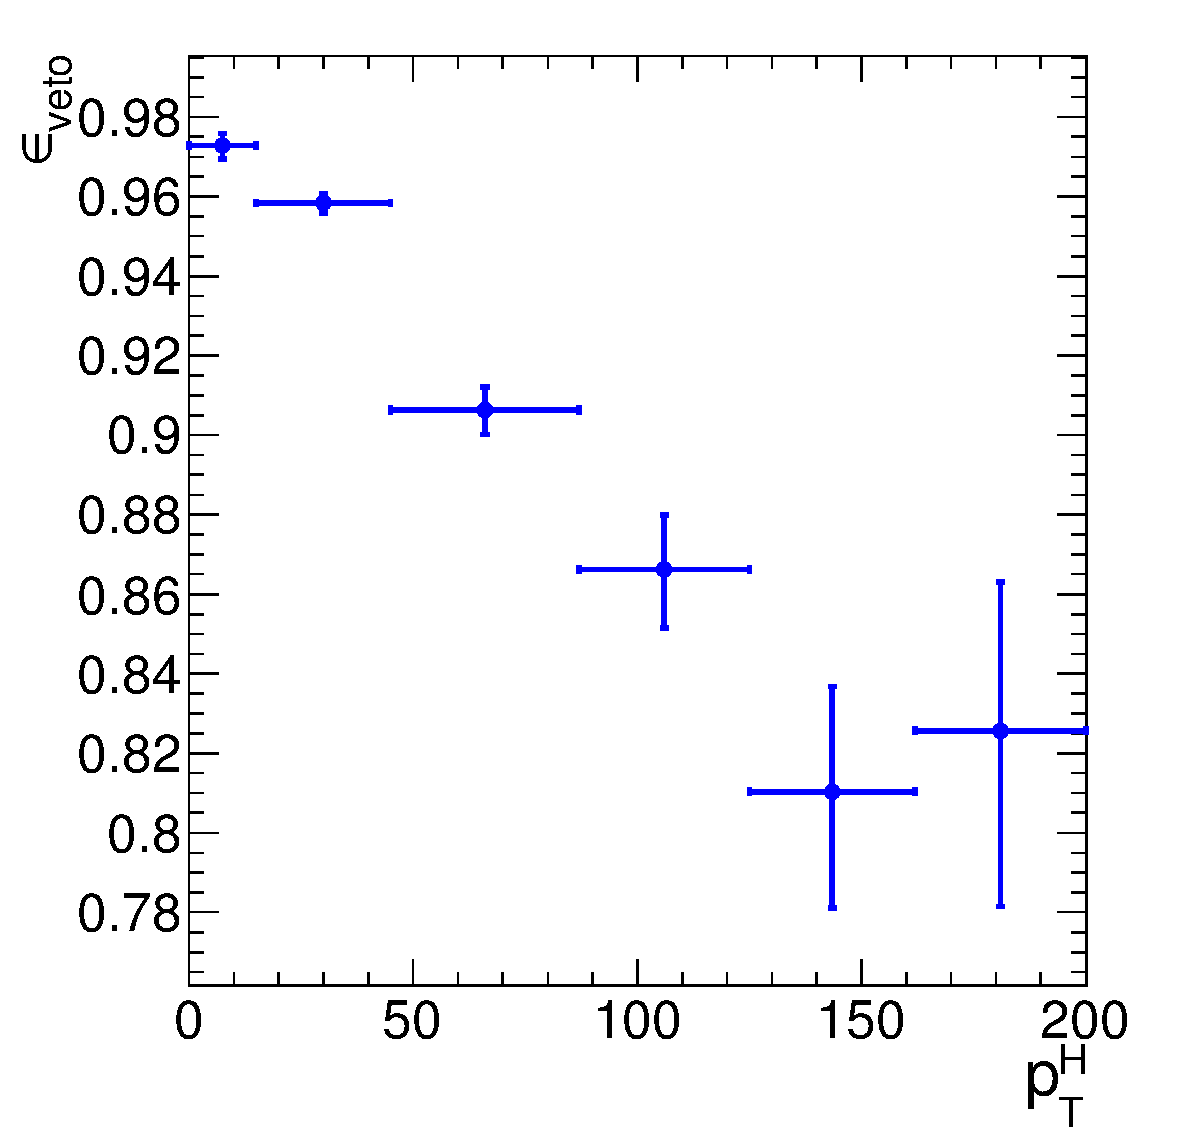
\includegraphics[width=0.4\textwidth]{images/eff_vs_pth.pdf}
	}
	\subfigure[]{
		\centering
		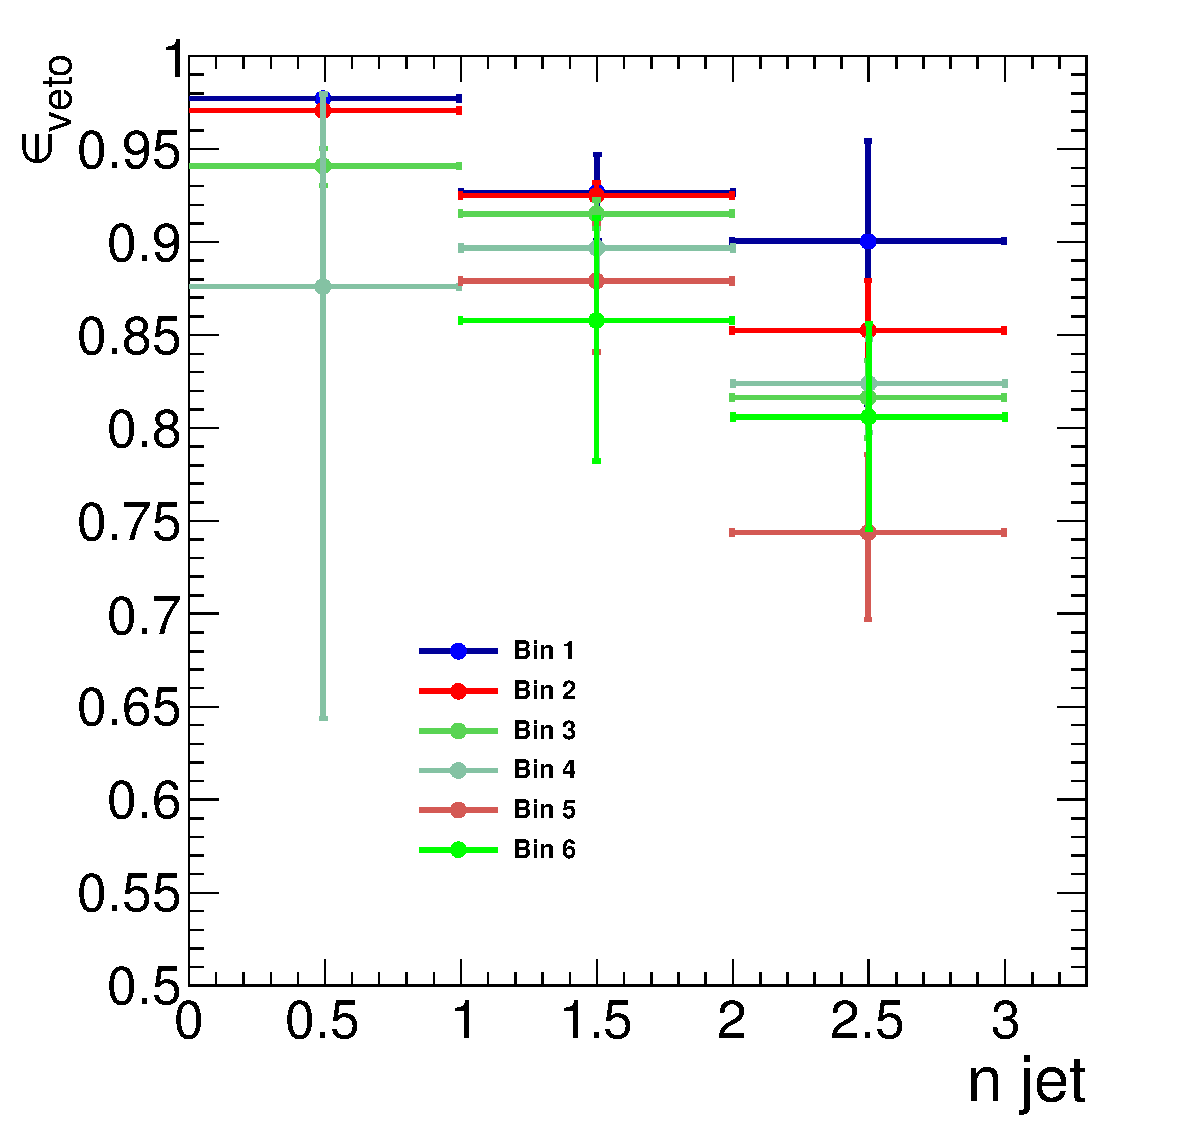
\includegraphics[width=0.4\textwidth]{images/eff_vs_jet.pdf}
	}
\caption{(a) Efficiency of the b tagging veto in different bins of \pth. (b) Efficiency of the b tagging veto in different bins of \pth, as a function of number of jets.}\label{fig:bveto_eff}
\end{figure}

\begin{comment}
\subsubsection{Jet multiplicity uncertainty} \label{subsec:stewart-tackman}

The jet bin uncertainty on the ggH production mode has been evaluated using the Stewart-Tackman method, following the recipe proposed in Refs.~\cite{Stewart:2011cf,Heinemeyer:2013tqa}.
Three independent nuisance parameters have to be associated with the inclusive ggH production cross sections $\sigma_{\geq 0}$, $\sigma_{\geq 1}$ and $\sigma_{\geq 2}$, which corresponds to the cross sections with $\geq 0$ jets, $\geq 1$ jet and $\geq 2$ jets respectively. According to the agreement on the treatment of uncertainties in the combination of ATLAS and CMS results~\cite{ATLAS:2011tau}, these nuisance parameters are labelled as \emph{QCDscale\_ggH}, \emph{QCDscale\_ggH1in} and \emph{QCDscale\_ggH2in}. However, in case the analysis is split in exclusive jet multiplicity bins, the jet bin uncertainties can be evaluated taking into account the correct correlations among the three nuisances following the Stewart-Tackman prescription.
Even though this analysis is inclusive in number of jets, the jet binning uncertainties must be included due to the presence of the b-jet veto, that introduces a dependency of the selection efficiency on the number of jets in the event. The veto efficiency has been evaluated in all the \pth bins defined in the analysis and as a function of jets multiplicity. The results are shown in Figs.~\ref{fig:veto_eff_pth} and \ref{fig:veto_eff_njet}. The drop of the veto efficiency at high values of \pth is due to the correlation with jets multiplicity.
	 	
\begin{figure}[htb]
\centering
	\subfigure[]{
		\centering
		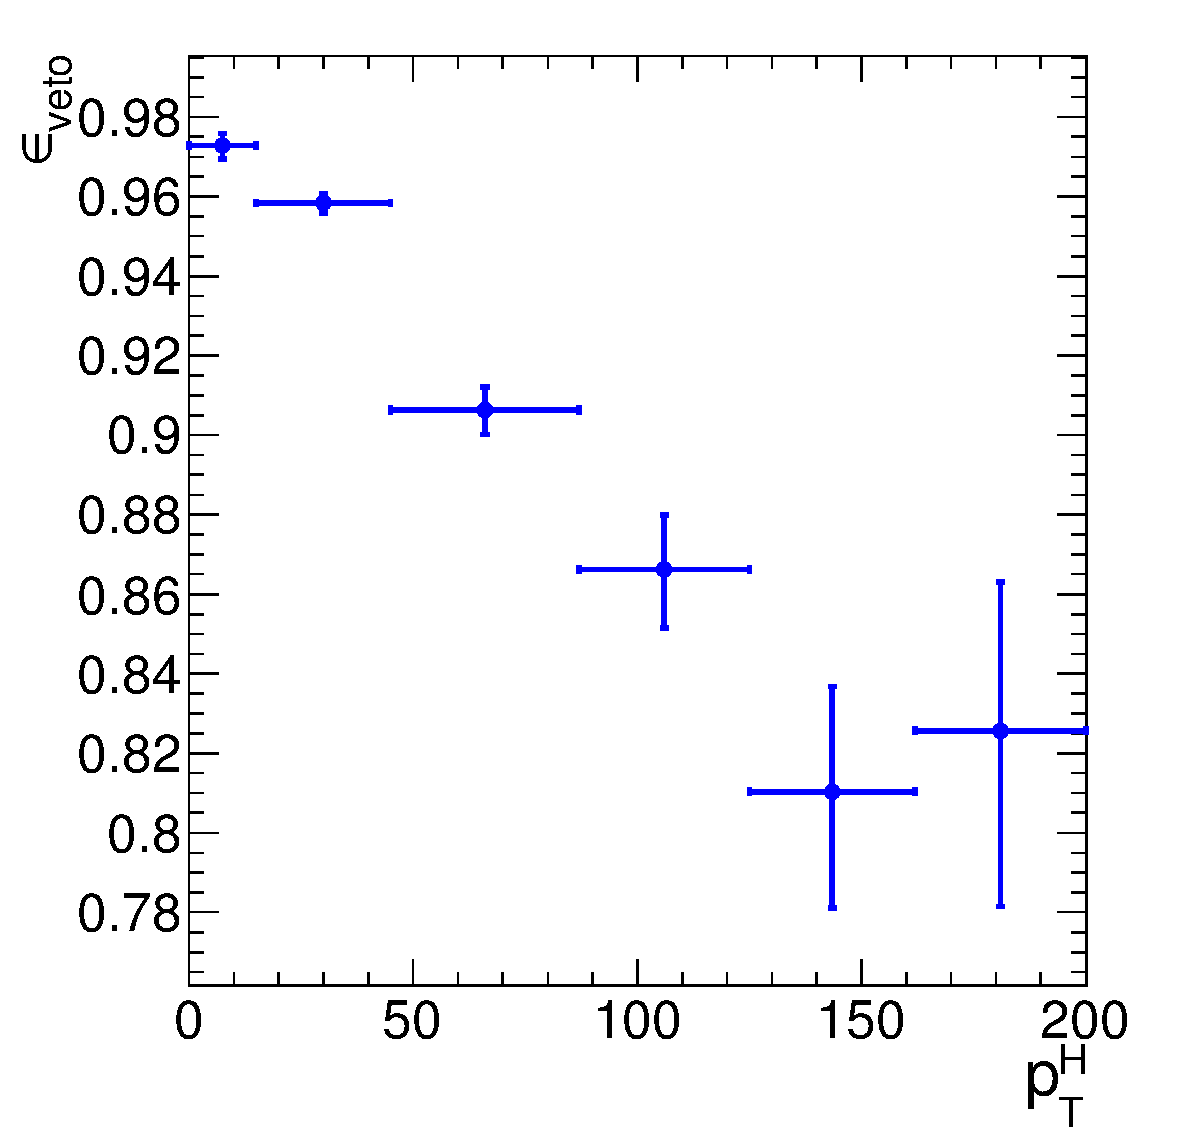
\includegraphics[width=0.45\textwidth]{images/eff_vs_pth.pdf}
		\label{fig:veto_eff_pth}
	}
	\subfigure[]{
		\centering
		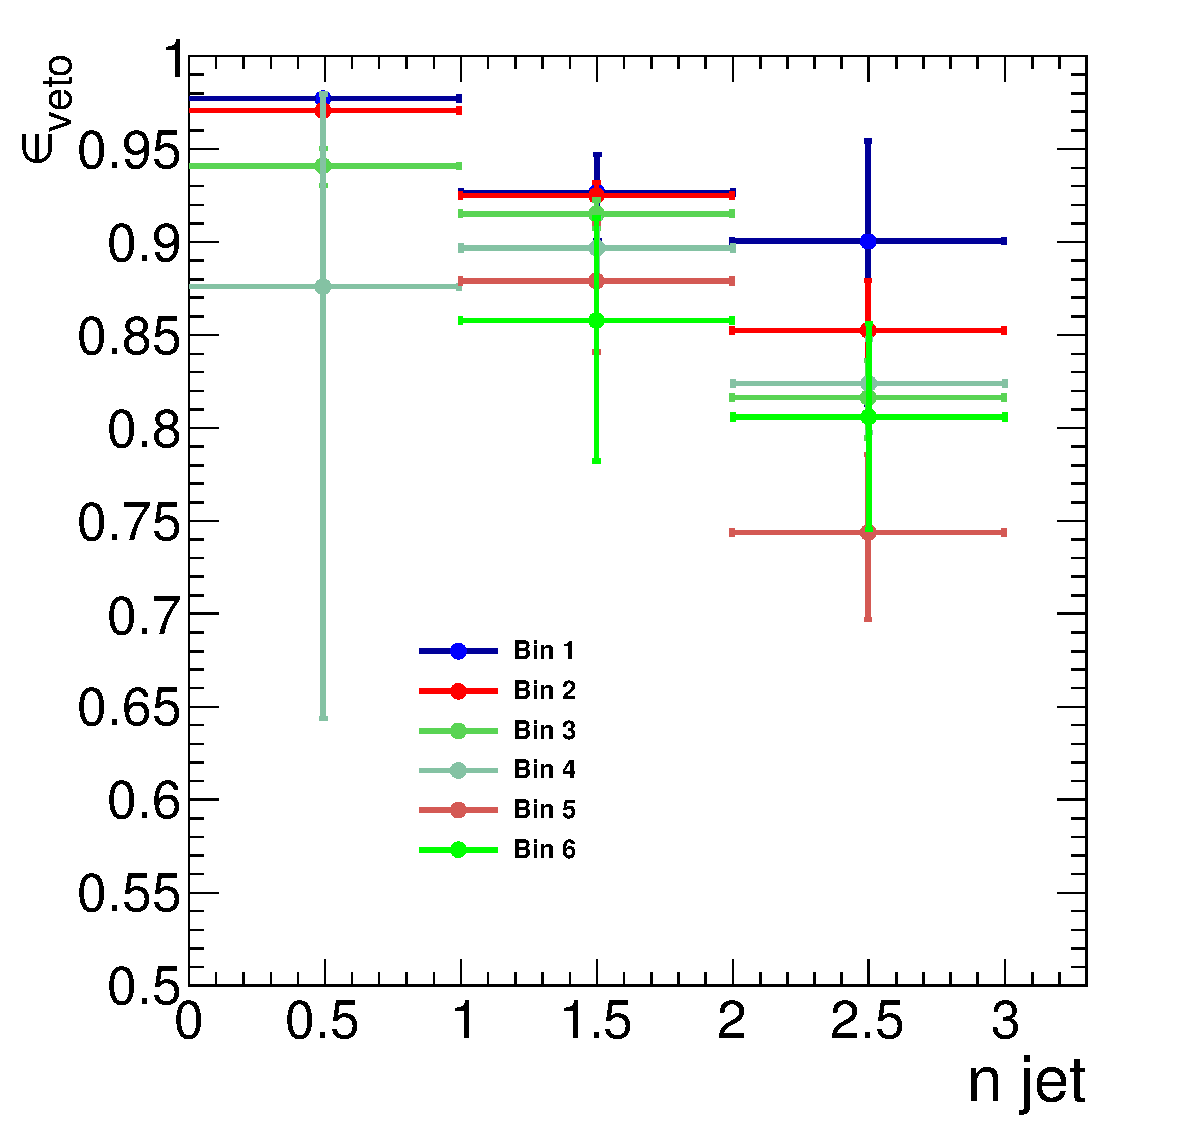
\includegraphics[width=0.45\textwidth]{images/eff_vs_jet.pdf}
		\label{fig:veto_eff_njet}
	}
\caption{(a) Efficiency of the b-tagging veto in different bins of \pth. (b) Efficiency of the b-tagging veto in different bins of \pth, as a function of number of jets.}\label{fig:bveto_eff}
\end{figure}

The first step of this procedure is to take the inclusive ggH cross section, $\sigma_\mathrm{ggH}$, and to convert the relative QCD up/down scale uncertainties, $\epsilon_+$ and $\epsilon_-$, to a log-normal uncertainty, i.e. $\kappa = \sqrt{\exp{(\epsilon_+)}\cdot \exp{(\epsilon_-)}}$. The exclusive cross sections, $\sigma_0$, $\sigma_1$ and $\sigma_2$, can be calculated starting from $\sigma_\mathrm{ggH}$ and using the selection efficiencies for the three jet bins. For every exclusive cross section the corresponding relative uncertainty is computed varying the renormalization ($\mu_R$) and factorization ($\mu_F$) scales independently of a factor 2 and $1/2$, and taking the cross section value corresponding to half of the maximum variation. The inclusive cross sections are then obtained summing the exclusive cross sections and propagating the uncertainties, i.e. $\sigma_{\geq 0 } = \sigma_0 + \sigma_1 + \sigma_2$, $\sigma_{\geq 1} = \sigma_1 + \sigma_2$, $\sigma_{\geq 2} = \sigma_2$.

The three nuisance parameters, including all the proper correlations among the jet bins, are defined according to Table~\ref{table:jet_binning_theory}, where the $f_n$ constants represent the exclusive theoretical $n$ jet bin fractions, i.e. $f_0 = \sigma_0/\sigma_{\geq 0}$, $f_1 = \sigma_1/\sigma_{\geq 0}$, $f_2 = \sigma_2/\sigma_{\geq 0}$.

\begin{table}[h]
\caption{Numerical calculation for the systematic uncertainties of jet binning.}
\label{table:jet_binning_theory}
\begin{center}
\begin{tabular}{|l|c|c|c|}
\hline
Nuisance parameter & 0-jet bin                                              & 1-jet bin                                            & 2-jet bin \\ 
\hline
&&& \\
QCDscale\_ggH          & $\Delta^0_{\geq 0} = (\kappa_{\ge 0})^{\frac{1}{f_0}} $    &      & \\ 
&&&\\\hline
&&&\\
QCDscale\_ggH1in       & $\Delta^0_{\geq 1} = (\kappa_{\ge 1})^{- \frac{f_1 + f_2}{f_0}} $ & $\Delta^1_{\geq 1} = (\kappa_{\ge 1})^{\frac{f_1 + f_2}{f_1}} $ & \\ 
&&&\\ \hline
&&&\\
QCDscale\_ggH2in        &                                                        & $\Delta^1_{\geq 2} = (\kappa_{\ge 2})^{- \frac{f_2}{f_1}} $     & $\Delta^2_{\geq 2} = (\kappa_{\ge 2})$ \\ 
&&&\\\hline

\end{tabular}
\end{center}
\end{table}

The nuisance parameters reported in table \ref{table:jet_binning_theory} have then been calculated for each \pth bin embedding the b-jet veto efficiency and using the following formulas:
\begin{equation}
\emph{QCDscale\_ggH}=\frac{\Delta^0_{\geq 0}\cdot f_{0}\cdot \varepsilon_{0}+\Delta^0_{\geq 1}\cdot f_{1}\cdot\varepsilon_{1}}{\Delta^0_{\geq 0}\cdot f_{0}\cdot \varepsilon_{0}+\Delta^0_{\geq 1}\cdot f_{1}\cdot \varepsilon_{0}} \quad,
\end{equation}
\begin{equation}
\emph{QCDscale\_ggH1in}=\frac{\Delta^1_{\geq 1}\cdot f_{1}\cdot \varepsilon_{1}+\Delta^1_{\geq 2}\cdot f_{2}\cdot \varepsilon_{2}}{\Delta^1_{\geq 1}\cdot f_{1} \cdot \varepsilon_{1}+\Delta^1_{\geq 2}\cdot f_{2}\cdot \varepsilon_{1}} \quad,
\end{equation}
\begin{equation}
QCDscale\_ggH2in=1 \quad,
\end{equation}
where $\varepsilon_0$, $\varepsilon_1$ and $\varepsilon_2$ are the selection efficiencies for the three jet categories.
These nuisance parameters are expected to be equal to one in case the efficiency is independent on the number of jets, i.e if $\varepsilon_0 = \varepsilon_1 = \varepsilon_2$.\\
The numerical values obtained following this procedure are reported in Table~\ref{table:jet_binning_meas} for each \pth bin.

\begin{table}[h]
\caption{Values of the jet binning nuisance parameters for different \pth bins.}
\label{table:jet_binning_meas}
\begin{center}
\begin{tabular}{ccccccc}
\toprule
\multirow{2}{*}{Nuisance parameter} & \multicolumn{6}{c}{\pth bin [GeV]} \\
& [0-15] & [15-45] & [45-85] & [85-125] & [125-165] & [165-$\infty$]\\
\midrule
QCDscale\_ggH  & 0.998  &   0.993  &   0.989  &   1.000  &   1.000   &  1.000 \\
QCDscale\_ggH1in &0.997   &  0.993  &   0.984  &   0.975 &    0.946 &    0.974  \\
\bottomrule
\end{tabular}
\end{center}
\end{table}
\end{comment}

%-------------------------------------------------------------------------------
\subsection{Statistics uncertainty of the simulated samples}
%-------------------------------------------------------------------------------

Due to the large range of weights used to correct the simulated distributions in order to
match those in data, the effective size of the simulated samples are sometimes smaller than
the actual number of events in the sample.
The uncertainties due to the finite statistics of the simulated samples are taken into account and propagated through the final result. Their effect on the signal strengths is found to be negligible.

%-------------------------------------------------------------------------------
\subsection{Treatment of systematic uncertainties in the analysis}\label{sec:syst_treatment}
%-------------------------------------------------------------------------------

As explained before, one can distinguish between normalization uncertainties, where a systematic effect is changing the normalization of a given process assuming the (\mll, \mt) shape is not affected, and shape uncertainties where the actual change in the (\mll, \mt) shape of the process is taken into account. The normalization uncertainties enter the analysis as constant normalization factors, whereas for shape uncertainties the nominal and the $+1\sigma$ and $-1\sigma$ shapes enter the analysis in form of three histograms with the same normalization. 

Effects of experimental uncertainties are studied by applying a scaling and smearing of certain variables related to physics objects, followed by a subsequent recalculation of all the correlated variables. This is done in simulation to account for possible systematic mis-measurements of the data. All experimental sources from Section~\ref{subsec:expsyst} but luminosity are treated both as normalization and shape uncertainties. For background with a data-driven normalization estimation, only the shape uncertainty is considered.
